\section{Theoretical Background}
High harmonic generation (HHG) is an optical phenomenon that involves nonlinear processes wherein laser light frequency is converted into multiple integer multiples. When atoms and molecules are exposed to intense laser fields, typically in the near-infrared range, harmonics of extremely high orders are produced.\cite{hhg-book} We will start by defining some plasma parameters. Then we will give a brief overview of the theory of HHG in gases, followed by a detailed discussion of HHG in plasma.

\subsection{Plasma Parameters}
\subsubsection{Underdense and Overdense Plasma}
Plasma frequency of a plasma with density $n_p$ is given by\cite{chen}
\begin{equation}
    \label{eq:plasma-frequency}
    \omega_p = \sqrt{\frac{n_p e^2}{\epsilon_0 m_e}}
\end{equation}
Let the frequency of the incident laser pulse be $\omega_l$. Now, if $\omega_l > \omega_p$, the plasma is called \textit{underdense}. In this case, the plasma is transparent to the laser pulse. On the other hand, if $\omega_l < \omega_p$, the plasma is called \textit{overdense}. In this case, the laser can not penetrate the plasma and is reflected back. The case $\omega_l = \omega_p$ corresponds to critical plasma and density in this case is called \textit{critical density} $n_c$. Using Equation \ref{eq:plasma-frequency} gives;
\begin{equation}
    \label{eq:critical-density}
    n_c = \frac{\epsilon_0 m_e \omega_l^2}{e^2}
\end{equation}

\subsubsection{Relativistic Laser Pulse}
For a laser of frequency $\omega_l$ and electric field amplitude $E_0$, the laser vector potential is defined as
\begin{equation}
    \label{eq:vector_potential}
    a_0 = \frac{eE_0}{m w_l c}
\end{equation}
A laser is called relativistic if $a_0 \ge 1$. In this situation, the intensity of laser becomes very high and it starts to drive the charged particle it interacts with by relativistic speeds.

\subsection{HHG in Gases}

HHG phenomena take place when gases are subjected to the influence of an intense laser pulse. The interaction leads to three different types of ionization, which are dependent on the intensity and frequency of the light. If the photon's energy is equal to or greater than the ionization potential of the atom, photon ionization will occur. On the other hand, if the laser's energy is lower than the ionization potential of the atom, multiphoton ionization and tunneling ionization will occur instead. The determination of multiphoton and tunneling ionization depends on the atomic ionization potential $I_p$, the laser frequency $\omega$, and the amplitude of the laser field strength $F$. In the multiphoton limit, the rate of ionization follows a power law, whereas in the tunneling limit, it increases exponentially as the field strength increases. The adiabaticity parameter, given by
\begin{equation}
    \label{eq:adiabatic}
    \gamma =\Omega \sqrt{2I_p/F}
\end{equation}
determines the boundary between multiphoton and tunneling ionization, with high values corresponding to multiphoton ionization and low values to tunneling ionization. To be precise, $\gamma^2 \gg 1$ corresponds to multiphoton ionization and $\gamma^2 \ll 1$ to tunneling ionization.\cite{gas-second}

\subsubsection{Three Step Model}

In three-step model, we treat the motion of electron initially using quantum mechanics. After it tunnel ionizes from the parent atom, we treat its subsequent dynamics classically. The HHG occurs in three steps:

\begin{figure}[H]
    \centering
    \subfloat[\centering Three steps and fields. The solid black line in the figure shows the binding potential well. The green line is the potential due to the laser field while the solid blue line is the potential created by the instantaneous laser field along with the binding potential well.]{{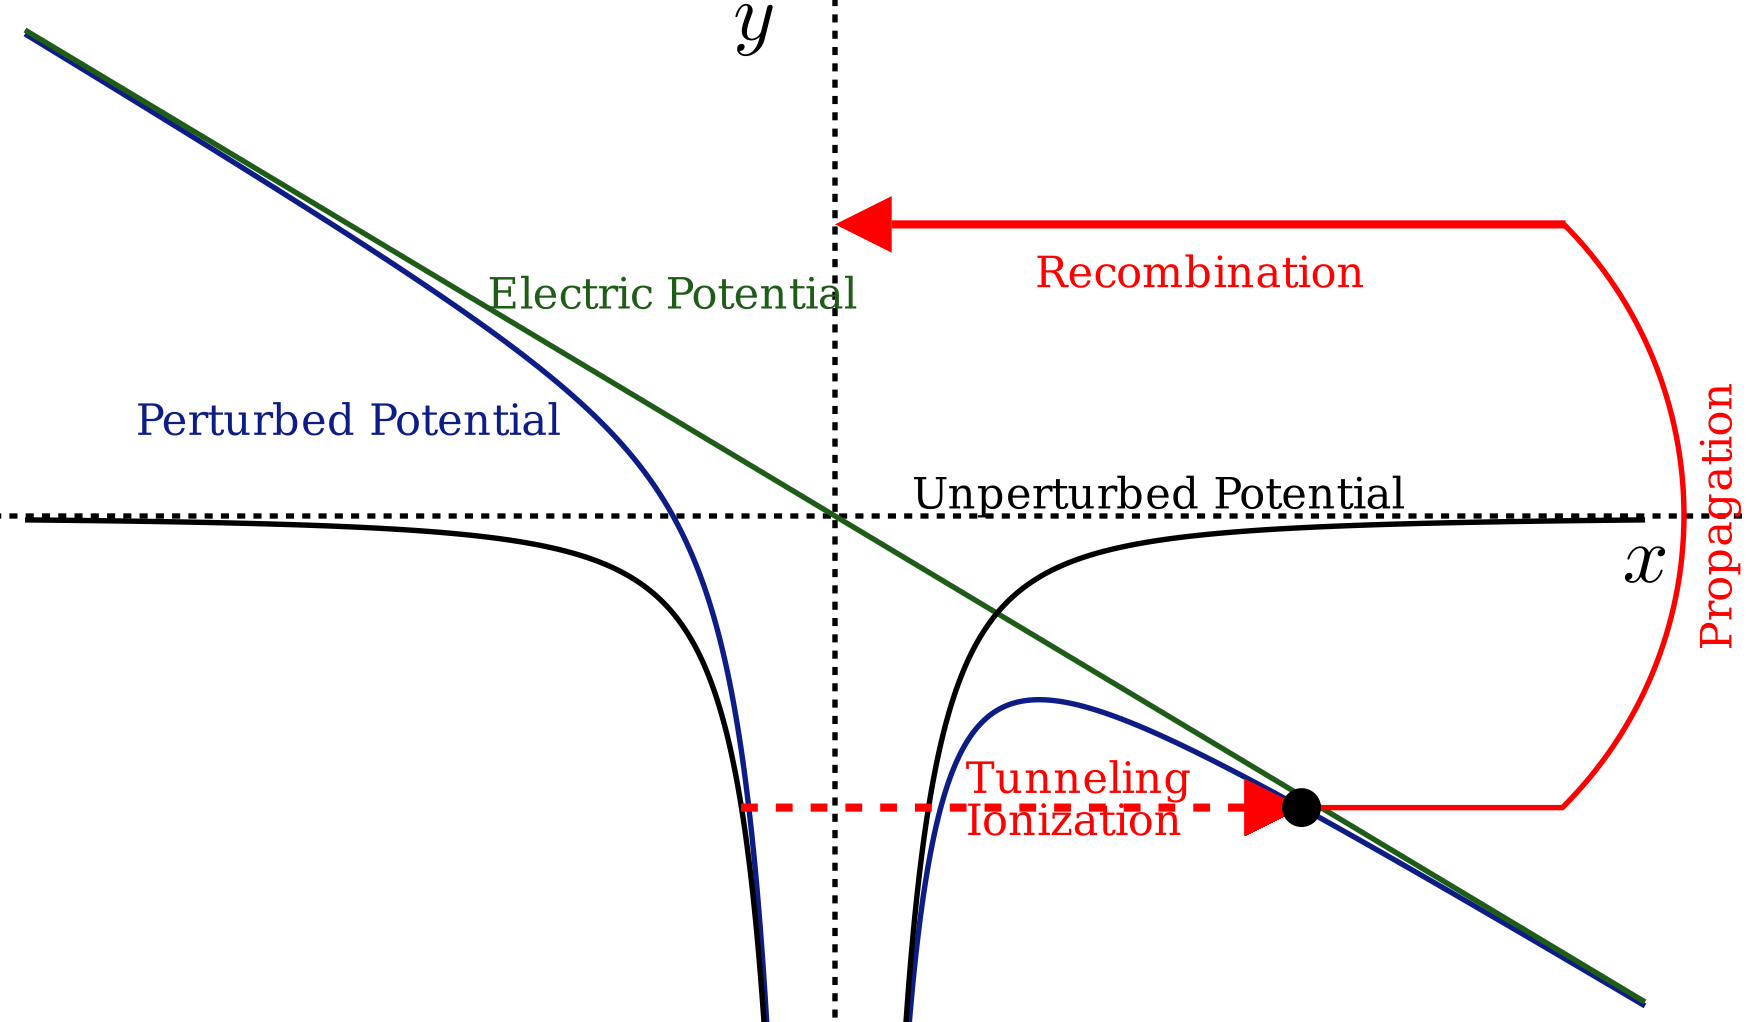
\includegraphics[width=0.47\textwidth]{three_step_one.png}}}%
    \quad
    \subfloat[\centering The wave functions of electrons (the red lines). Initially, it is in a potential well. While tunneling, the wave function decay exponentially. After the electron has tunneled through the barrier, it behaves like a free particle with a wave function specified by a smaller amplitude.]{{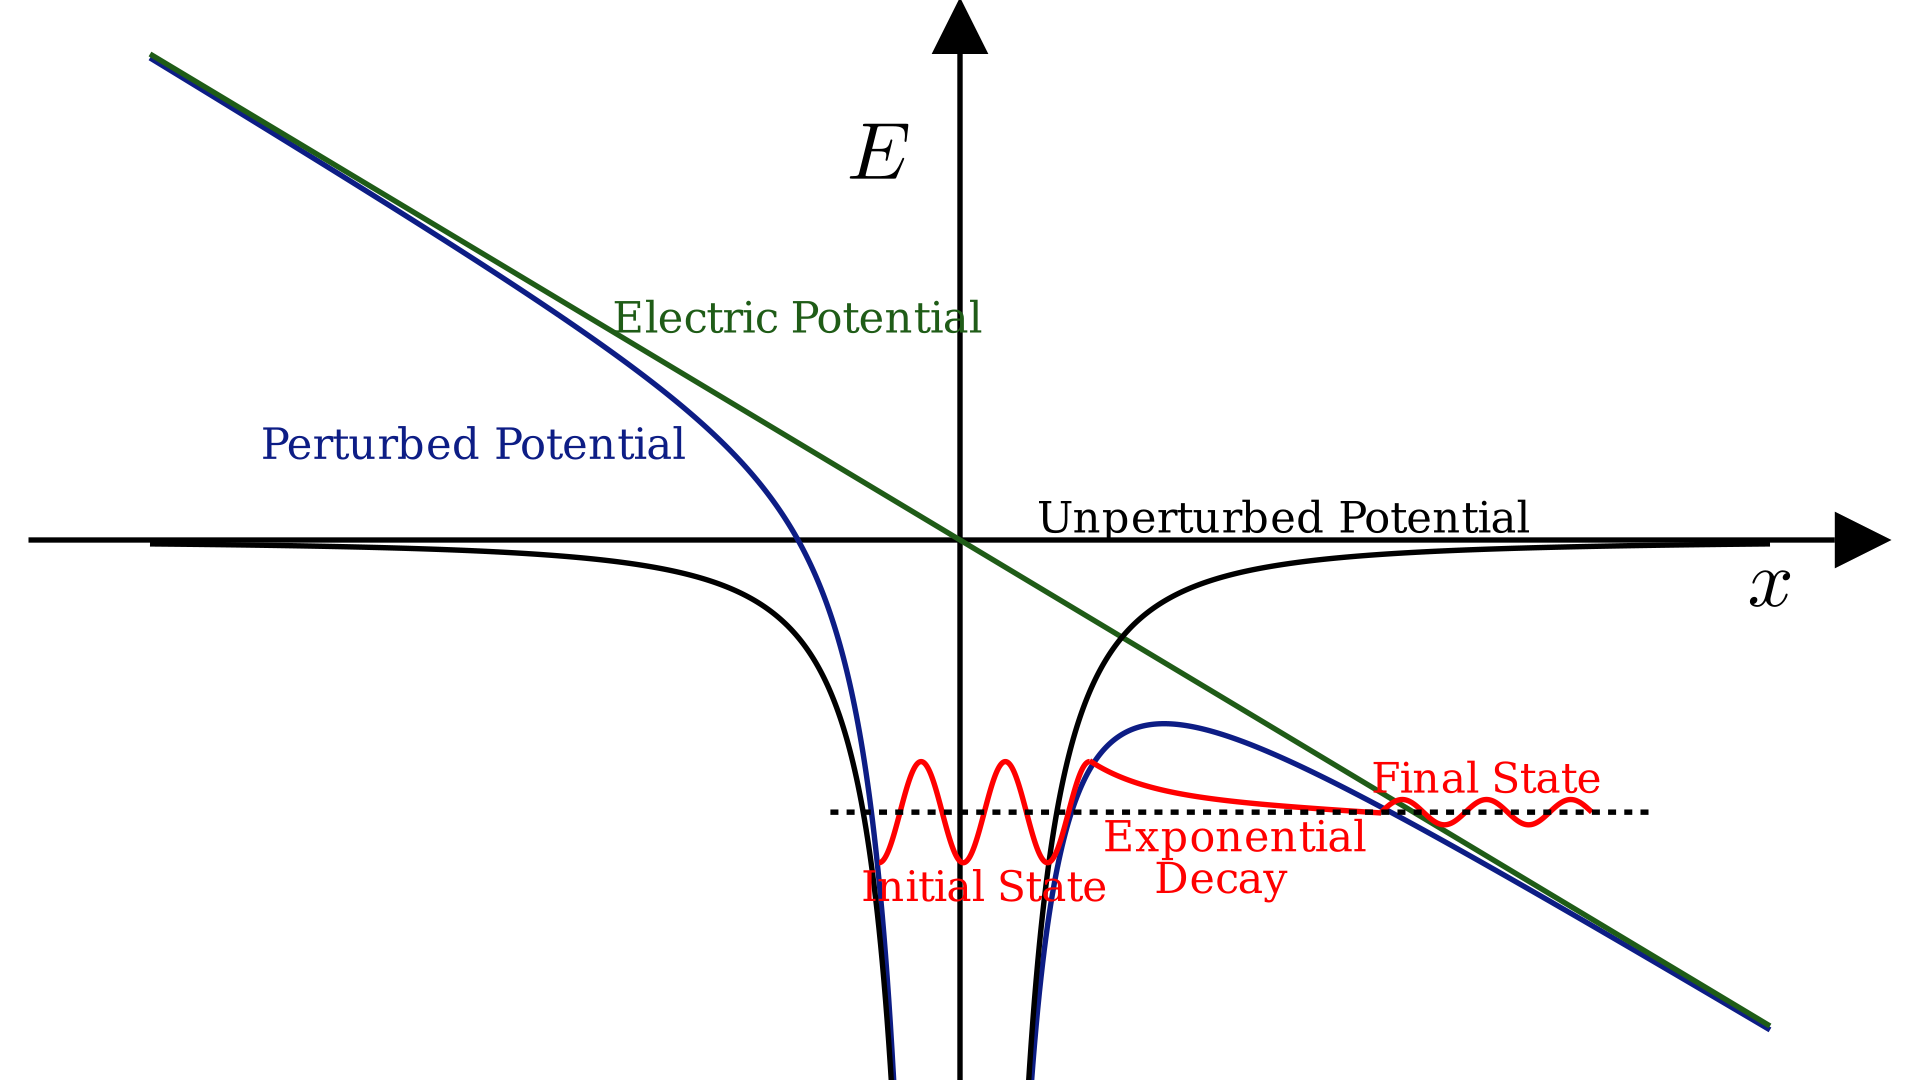
\includegraphics[width=0.47\textwidth]{three_step_two.png}}}%
    \caption{The Three Step Model}%
    \label{fig:three-step}%
\end{figure}

\begin{enumerate}
    \item \textbf{Tunnel ionization} The laser field, which we have assumed to be linearly polarized along the $x$-axis, gives a potential in the form of \(\hat V_L(t)-xFcos(\omega_Lt)\), that is, the potential is proportional to $-x$. This is drawn in figure \ref{fig:three-step} (a) as the green line. When this potential couples with the original potential well (in the black line), the potential is deformed (the blue line), called barrier suppression. Electron tunnels through this potential well.
    \item \textbf{Free propagation in the presence of the field} After tunneling, the electron is considered to have no initial velocity as it enters the vacuum. It then experiences acceleration from the electric field of the laser beam. About half a cycle after being ionized, the electron changes direction and moves back toward the parent nucleus due to the reversal of the electric field's direction. During this process, the electron continues to be accelerated.
    \item \textbf{Recollision and recombination} Next, the electron will collide with the nucleus which is the recombination process. During recombination, while the electron returns to its ground state, it can emit radiation of frequency that are multiple of the laser intensity. This is how high harmonics are generated.
\end{enumerate}

\subsection{HHG in Plasma}
The spectrum from HHG consists of several of integer harmonics of the incident laser pulse (with their intensities decreasing), followed by a plateau, a region, where the harmonic intensity is almost constant over many orders and finally a sharp cutoff. Several of models and theories have been proposed explaining this power law and cutoff. Bezzerides et al.\cite{hhg-relativistic} gave the first model way back in 1983. Their model was based on the relativistic equation of motion and hydrodynamics approximation. They found a cutoff frequency as
\begin{equation}
    \label{eq:cutoff-relativistic}
    n_{\max}^2 = \frac{n_p}{n_c}
\end{equation}
where $n_p$ is the plasma density and $n_c$ is the critical density. The authors showed that the main cause of high-harmonic emission is the powerful nonlinear restoring force that arises during resonant absorption in a density profile that is extremely steep. However, this model was not able to explain the plateau region as well as the fact that we get harmonics that are much higher than the cutoff frequency given by Eq. \ref{eq:cutoff-relativistic}.

\subsubsection{Oscillating Mirror Model}
The concept underlying this model is that the incident laser field results in a periodic oscillation of the surface of the plasma mirror relativistic speeds. This oscillating mirror at relativistic speeds results in a periodic Doppler effect on the reflected field, which is responsible for the occurrence of HHG. In this model, it is assumed that the duration of the light pulse is very brief and hence one can ignore the motion of the ions. The ions are considered as a static positive background charge. Additionally, the details of changes in the electron density profile are ignored, and the collective motion of the electrons is represented by the motion of the boundary of the supercritical region. This boundary serves as an effective reflective surface that undergoes oscillatory motion, which is referred to as the oscillating mirror. Using these assumptions, we follow von der Linde et al.\cite{hhg-main} to derive the spectrum of HHG. First, we show that the HHG can be understood as a phase modulation due to the moving mirror.

Assuming retardation can be disregarded for the time being, the reflected wave suffers a phase shift due to the periodic sinusoidal motion of the reflecting surface (the PM) along the z-direction. This can be determined:

\begin{equation*}
    s(t) = s_0 \sin(\omega t)
\end{equation*}

is given by
\begin{equation*}
    \phi(t) = (2\omega_0s_0/c)\cos\alpha \sin \omega_m t
\end{equation*}

$\alpha$ being the angle of incidence while $\omega_m$ is the mirror frequency (the frequency at which modulation occurs). The reflected wave has the elecctric field as:

\begin{equation}
    E_R \propto e^{-i\omega_0 t}e^{i\phi(t)} =  e^{-i\omega_0 t} \sum _{n \to -\infty}^{n \to -\infty}J_n(\chi) e^{-in\omega_m t}
\end{equation}

with $J_n(\xi)$ being the $n^{\text{th}}$ order Bessel function and
\begin{equation}
    \label{eq:chi-def}
    \chi = \frac{2\omega_0s_0\cos\alpha}{c}
\end{equation}

Depending on the polarisation and incidence angle of the incident light, the reflecting surface experiences periodic motion with a frequency of $2omega_0$ or a superposition of $omega_0$ and $2omega_0$. In consequence, the modulation frequencies produced by the mirror motion are $omega_m = omega_0$ and/or $omega_m = 2omega_0$. This form of modulation produces sidebands that represent even and odd harmonics of the fundamental frequency $omega_0$. These ideas propose an explanation for the generation of high-order harmonics at the plasma-vacuum interface as phase modulation from an intermittently moving reflecting surface.

\subsubsubsection{p- and s-Polarization}\label{section:selection}
\begin{figure}[H]
    \centering
    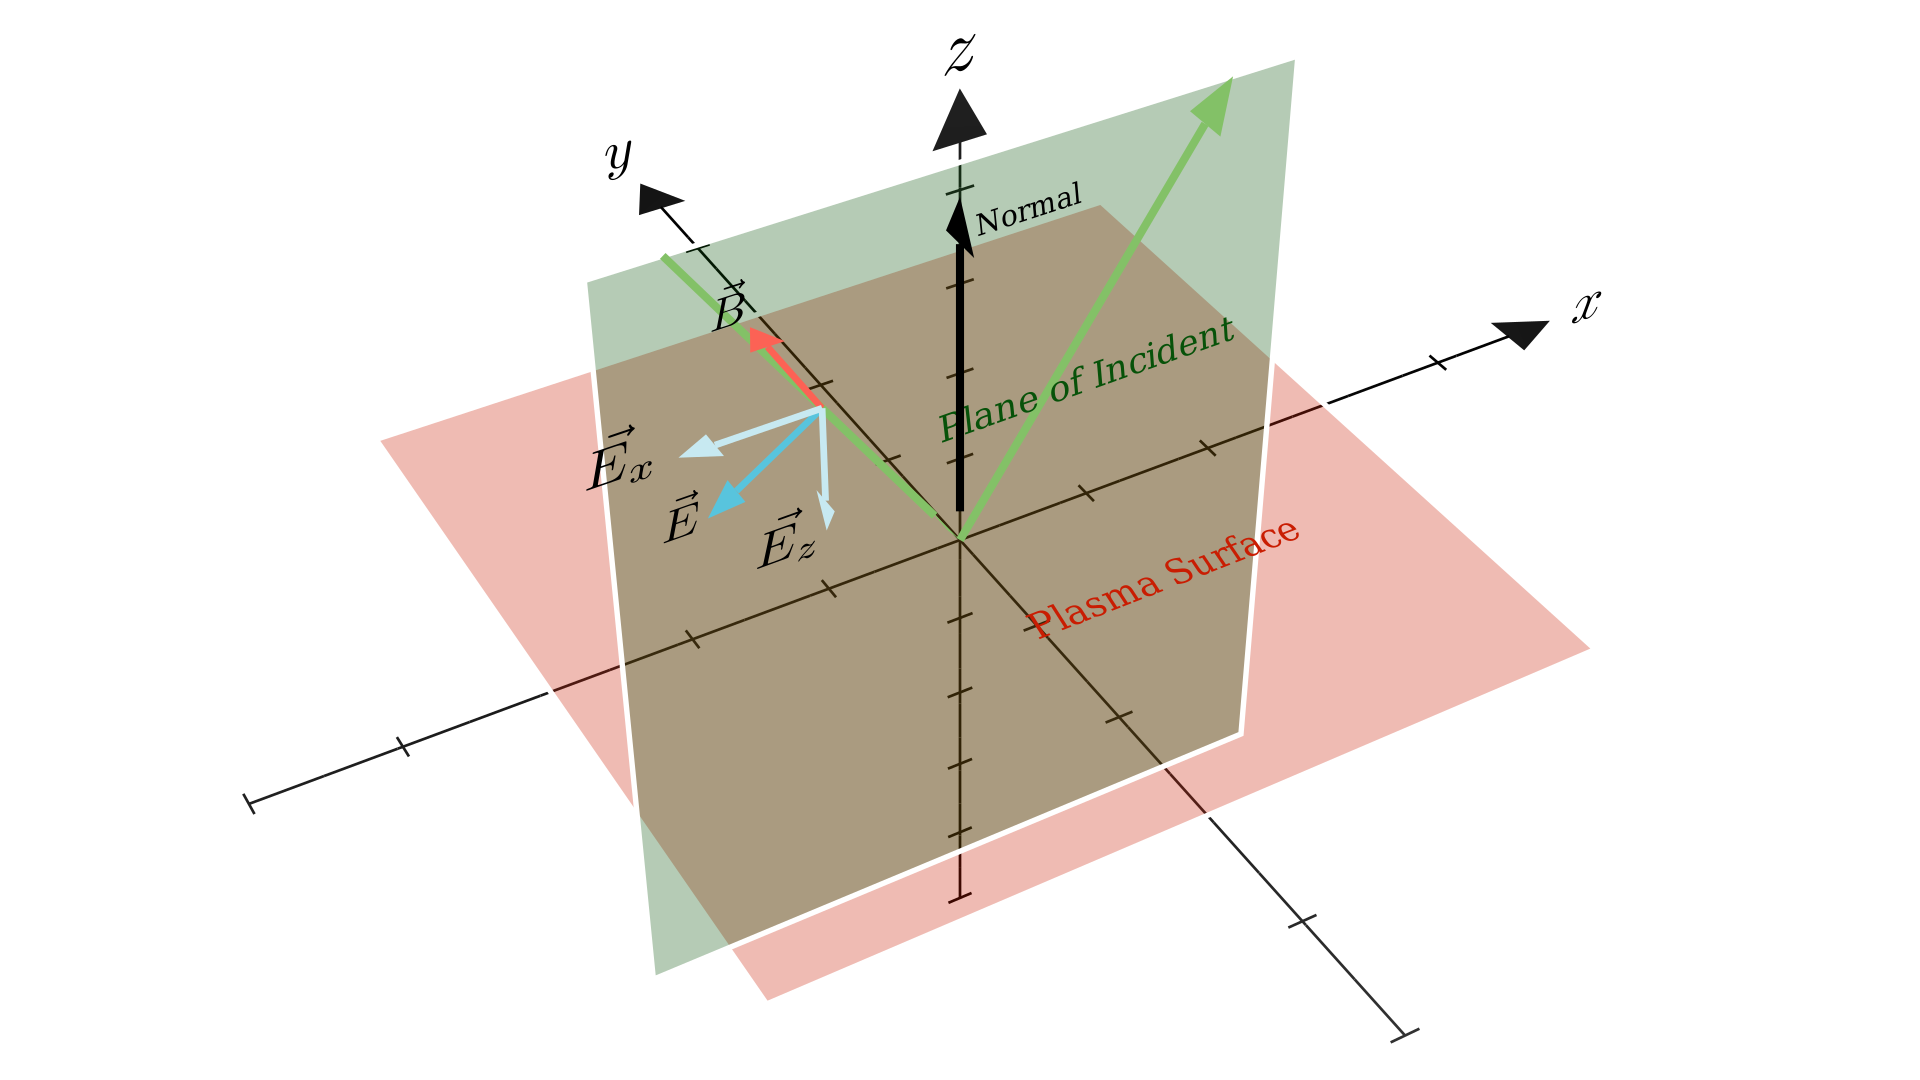
\includegraphics[width=0.8\textwidth]{p.png}
    \caption{p-polarization. The electric field is parallel to the plane of incidence while the magnetic field is perpendicular to the plane of incidence and hence the motion of the electron occurs within the plane of incidence.\\All the illustrations in this sections, if not stated otherwise, are made by the authors using manim\cite{manim}.}
    \label{fig:p-polarized}
\end{figure}

\begin{itemize}
    \item \textbf{p-Polarized Light}: In this case, the electric field is parallel to the plane of incidence while the magnetic field is perpendicular to the plane of incidence and hence the motion of the electron occurs within the plane of incidence. The electron boundary is driven at frequencies $\omega_0$ and $2\omega_0$, as both the transverse and longitudinal components of the electron velocity contribute to the motion of the boundary. As a result, both even and odd harmonics with p-polarization are produced in this scenario. Please refer to the Figure \ref{fig:p-polarized}.
    \item \textbf{s-Polarized Light}: Here, the electric field is parallel to the plasma-vacuum interface and of the magnetic field is perpendicular. This means that the electrons will move in a plane perpendicular to the plane of incidence. In this setup, only the longitudinal component of the electron motion contributes to the mirror motion, while the transverse component is ineffective. Consequently, the mirror motion is driven at a single frequency, $\omega_m = 2\omega_0$. As a result, the reflected light consists of odd harmonics with s-polarization and even harmonics with p-polarization. Please refer to the Figure \ref{fig:s-polarized}.
          \begin{figure}[H]
              \centering
              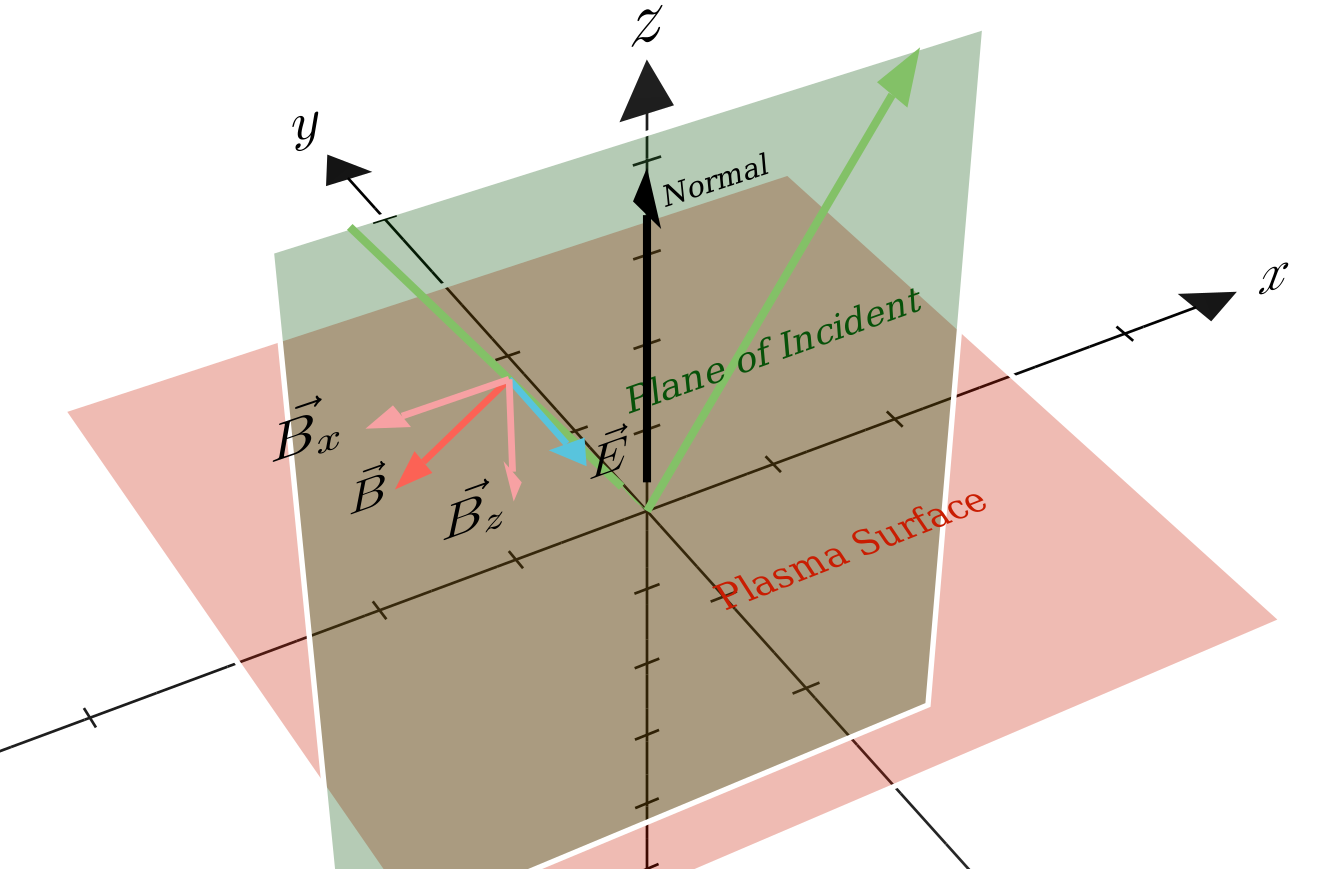
\includegraphics[width=0.8\textwidth]{s.png}
              \caption{s-polarization. The electric field is parallel to the plasma-vacuum interface. This means that the electrons will move in a plane perpendicular to the plane of incidence.}
              \label{fig:s-polarized}
          \end{figure}
\end{itemize}

\begin{table}[h]
    \centering
    \caption{Selection Rule for Polarization}
    \vspace{0.5cm}
    \label{tab:selection-rule}
    \begin{tabular}{|l|l|l|}
        \hline
                                         & \textbf{s-polarized Harmonics} & \textbf{p-polarized Harmonics} \\ \hline
        \textbf{s-Polarized Fundamental} & Odd                            & Even                           \\ \hline
        \textbf{p-Polarized Fundamental} & None                           & Odd and Even                   \\ \hline
    \end{tabular}
\end{table}

\subsubsubsection{HHG Spectrum}
We chose the coordinate system shown in Fig. \ref{fig:s-polarized}. The incident light is polarized along the $y$-axis. The incident light has electric field in the form of:
\begin{equation*}
    E(t, x, z) = E_0 \exp\left(-i\omega_0\left(t-x/c \sin\alpha - z/c \cos\alpha\right)\right)
\end{equation*}

We assume the surface oscillations to be of the form:
\begin{equation*}
    s(t) = s_0 \sin\left( \omega_m \left(t - x/c \sin\alpha\right) \right)
\end{equation*}

The maximum displacement of the surface is $s_0$ is bounded and it is determined by the fact that the velocity must not exceed the speed of light $c$. For example, for s-polarization, as $\omega_m = 2 \omega_0$, we have
\begin{align*}
    s_0 < \frac{c}{\omega_0} & = \frac{c}{2\omega_0} \\
    \therefore \chi          & < \cos\alpha
\end{align*}

For our analysis, we will make the assumption that we ca express the reflected wave as a plane wave which is propagating in the direction of specular reflection. This type of wave has form:

\begin{equation*}
    E_R = G(t - x/\sin\alpha + z/\cos\alpha) = G(u)
\end{equation*}

If we assume that the reflecting surface is perfectly reflecting, the function $G(u)$, defined above, can be determined by the boundary condition that the net field must vanish at the reflecting surface, given $z = s(t,x)$. This condition can be expressed as:

\begin{equation}
    \label{eq:bc}
    E(t,x,s(t,x)) + E_R(t,x,s(t,x)) = 0
\end{equation}

We observe that both the sides of the Eq. \ref{eq:bc} are function only of $\xi = t - x/c \sin\alpha$. The spectrum of the reflected wave can be obtained by using the Fourier transform of $G(u)$:
\begin{equation*}
    G(\omega) = \int_{-\infty}^{\infty} G(u) e^{-i\omega u} du
\end{equation*}

where $u = \xi - s_0/c \cos\alpha \sin(\omega_m \xi)$ Integrating, this comes out to be:
\begin{equation}
    \label{eq:G_omega}
    G(\omega) = -2 \pi E_0 \sum_{-\infty}^{+\infty} \frac{1}{1+ n\omega_m /2 \omega_0} \times J_n \left(\left( 1+ n\omega_m /2\omega_0\right)\xi\right)\delta \left(\omega - \omega_0 - n\omega_m\right)
\end{equation}

with $J_n$ being the the Bessel function of order n.

\begin{figure}[h]
    \centering
    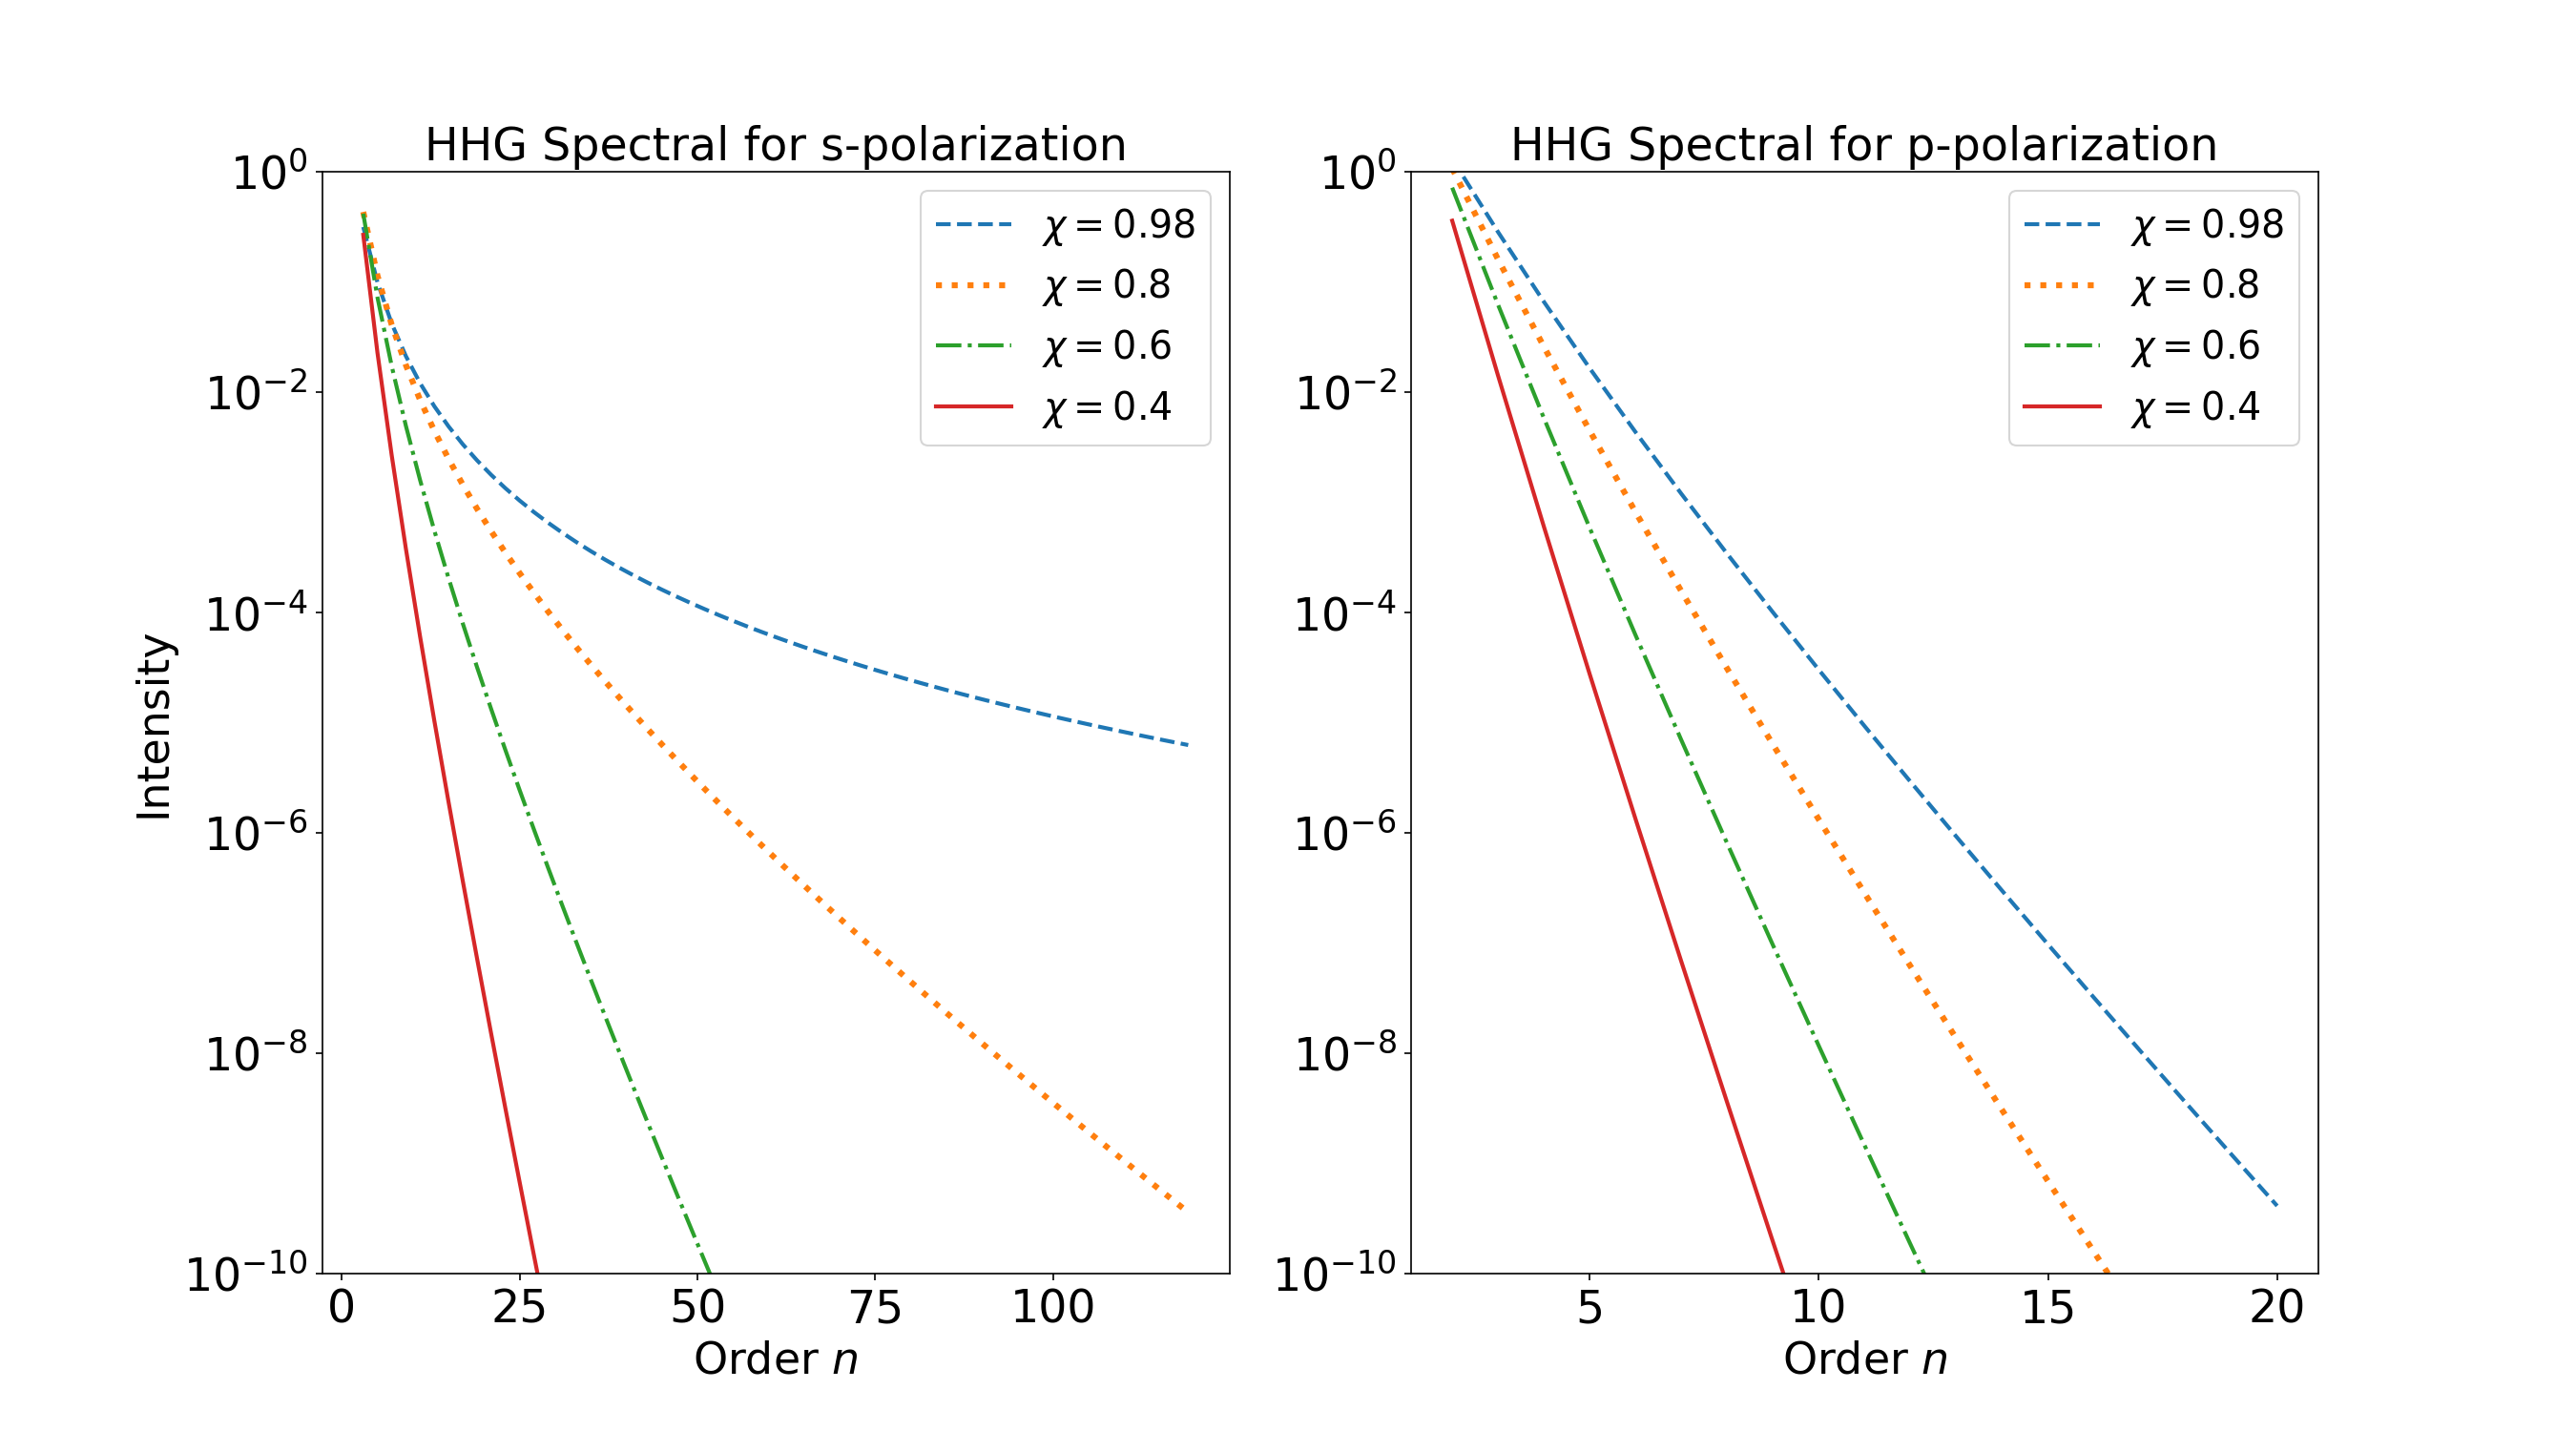
\includegraphics[width=0.85\textwidth, height=7cm]{spectrum.png}
    \caption{HHG spectrum for s and p polarization. The amplitudes of HHG is decreasing more rapidly for p-polarization than s-polarization}
    \label{fig:spectrum}
\end{figure}

For an s-polarization we have, $\omega_m = 2 \omega_0$ and hence equation \ref{eq:G_omega} reduces to:
\begin{equation}
    \label{eq:s-spectrum}
    S((2n+1)\omega_0) = (\pi E_0)^2\left(\frac{J_n((n+1)\xi)}{(n+1)}- \frac{J_{n+1}(n\xi)}{(n)}\right)^2
\end{equation}

For a p-polarization:
\begin{equation}
    \label{eq:p-spectrum}
    S(n\omega_0) = (\pi E_0)^2\left(\frac{J_{n-1}(\frac{1}{2}(n+1)\xi)}{\frac{1}{2}(n+1)}- \frac{J_{n+1}\frac{1}{2}((n-1)\xi)}{\frac{1}{2}(n-1)}\right)^2
\end{equation}

A plot of the spectra is shown in figure \ref{fig:spectrum}.
\subsubsection{Universal Spectra}
The \textit{ideal mirror} assumptions made by von der Linde et al.\cite{hhg-main} are not held in practice. In fact, an ideal mirror is not physically possible. Gordienko et al.\cite{universal-spectra} showed that it is not necessary to assume a form of plasma surface oscillation if the goal is just to get the cutoff and power law of the HHG spectrum. Assuming only the boundary condition equation \ref{eq:bc} and the periodicity of the surface motion, they found the following results which are valid for any type of plasma surface motion:
\begin{enumerate}
    \item The power law for monochromatic wave
          \begin{equation}
              \label{eq:power-law-u}
              I_n \propto 1/n^{5/2}
          \end{equation}
    \item The power law for broadband wave
          \begin{equation*}
              I_n \propto 1/n^{5/2}
          \end{equation*}
    \item The cutoff
          \begin{equation}
              \label{eq:cutoff-u}
              n_c \propto 4\gamma_{\max}^2
          \end{equation}
\end{enumerate}
